\chapter{Use cases}\label{ch:usecases}

\begin{figure}[p]
	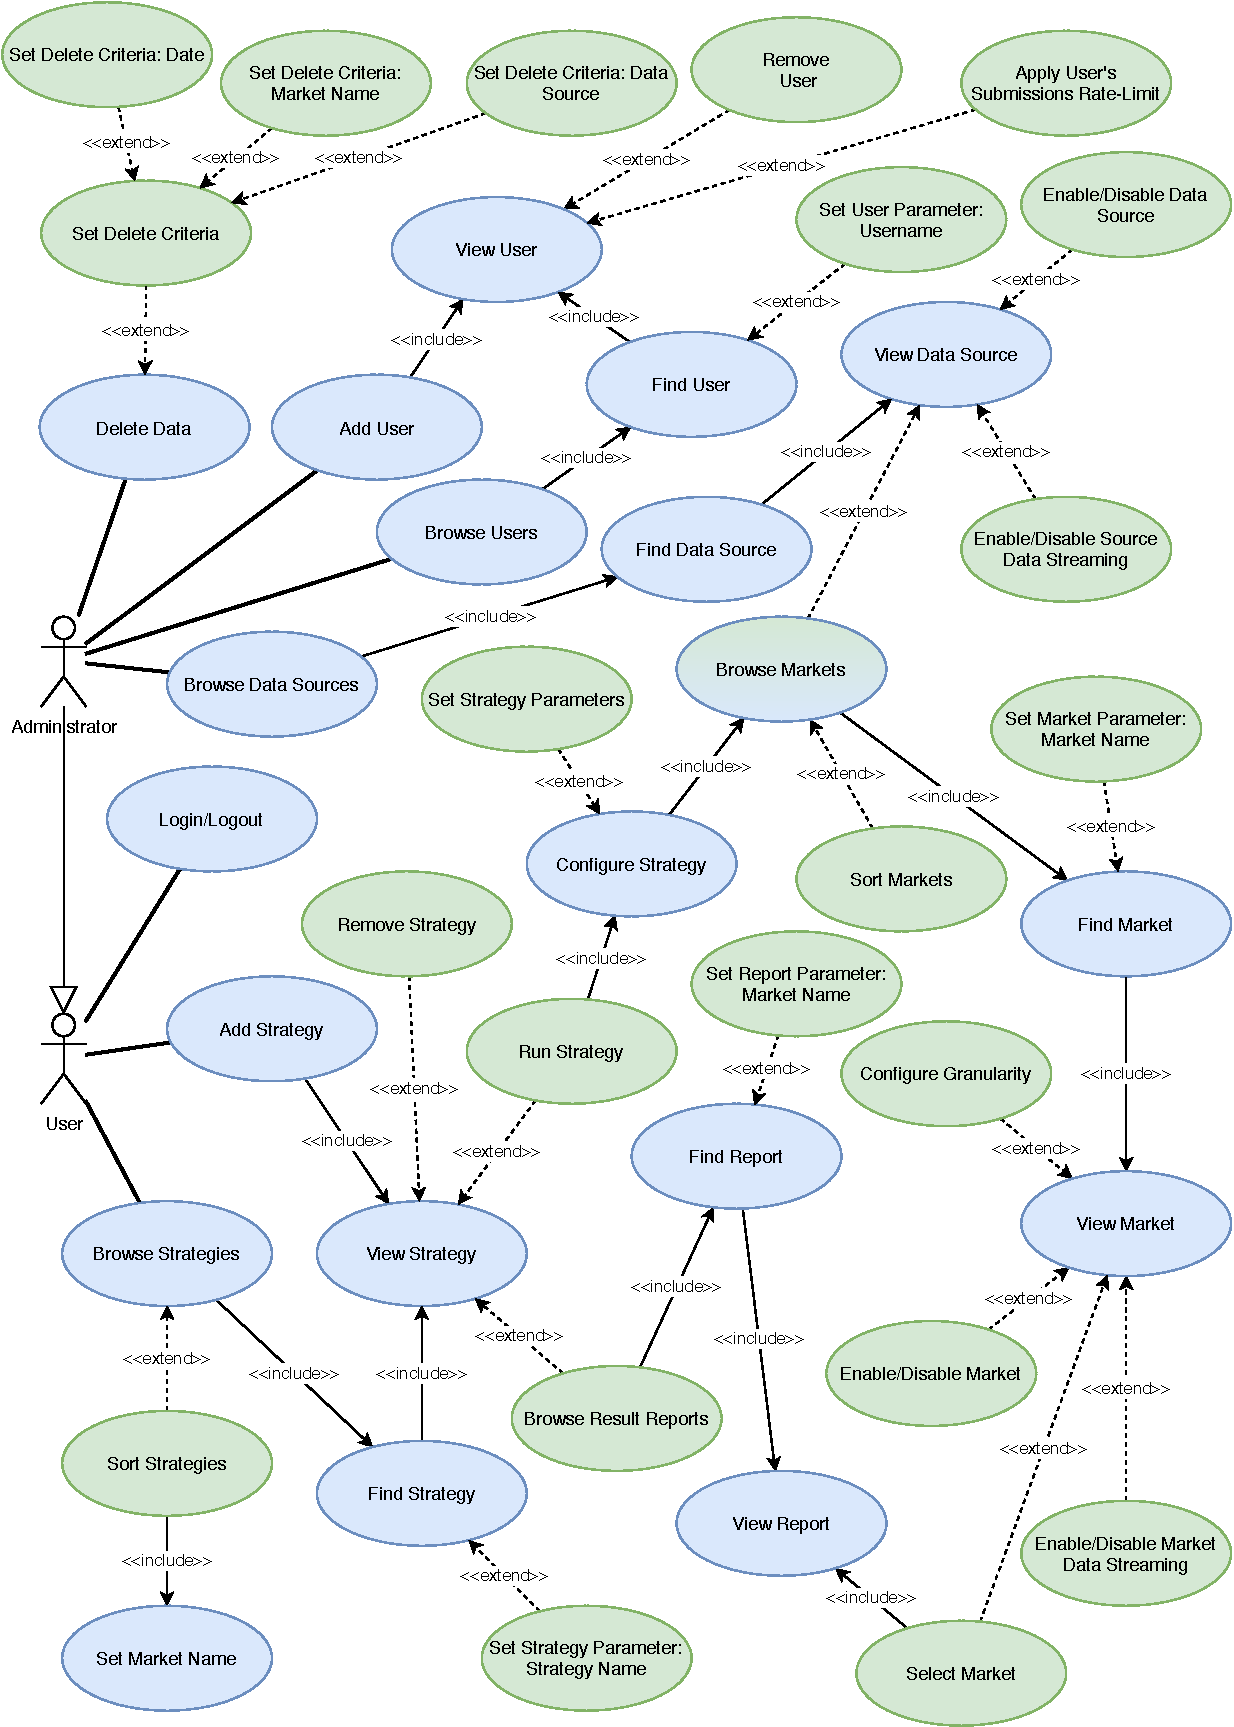
\includegraphics[width=\textwidth]{usecases}
	\caption{Use cases UML diagram.}\label{fig:usecases}
\end{figure}

\figref{fig:usecases} shows the UML diagram for use cases.

The following use cases are defined (all use cases, except Login, requires the
user to be logged in):
\begin{description}
	\item[Login/Logout] A user can login in the application using its
		credentials (username, password). When logged in, he can logout
		from the application at any time;
	\item[Add Strategy] Add a new strategy, providing its implementation and
		a descriptive name;
	\item[View Strategy] See all the information about a strategy;
	\item[Run Strategy] Users can execute the selected strategy with the
		specified configuration;
	\item[Configure Strategy] Configure the strategy for the execution;
	\item[Set Strategy Parameters] Set the parameters used by the strategy;
	\item[Browse Markets] See the list of all markets (optional action for
		the administrator; required action for the user when he
		configures the strategy for execution);
	\item[Find Market] Search a market from the list, searching by market
		name;
	\item[View Market] Users can view a market to select it; the
		administrator can view and edit the configuration of the market;
	\item[Enable/Disable Market Selection] \textit{(admin)} Enable or
		disable the ability for users to select the market to run
		strategies over it;
	\item[Enable/Disable Market Data Sync] \textit{(admin)} Enable or
		disable the synchronization of the data from the source for the
		market;
	\item[Configure Granularity] \textit{(admin)} Set the minimum
		granularity of the selected market. The API scraper will
		download data using this granularity;
	\item[Select Market] Select the market for the execution of the
		strategy;
	\item[Browse Result Reports] See all reports of the executions of the
		selected strategy made by any user;
	\item[Find Report] Select a report from the list;
	\item[View Report] See all the statistics collected in the selected
		report;
	\item[Browse Strategies] See the list of all strategies saved in the
		application;
	\item[Sort Strategies] Sort strategies by their performance in a
		specific market;
	\item[Find Strategy] Search a strategy by name;
	\item[Download Strategy] Download the file containing the strategy's
		code;
	\item[Remove Strategy] Delete a strategy (A user can delete only
		strategies he created, except for the administrator that can
		delete any strategy);
	\item[Add User] \textit{(admin)} Add a new user for the application,
		specifying its username and password;
	\item[Browse Users] \textit{(admin)} See the list of all the users of
		the application;
	\item[Find User] \textit{(admin)} Search a user by its username;
	\item[View User] \textit{(admin)} See all the information about the
		selected user (except the password);
	\item[Remove User] \textit{(admin)} Delete a user from the application;
	\item[Delete Data] \textit{(admin)} Delete data which satisfy some
		criteria \exgratia{old data; data of a specific market or data
		source, \etc};
	\item[Browse Data Sources] \textit{(admin)} See the list of all data
		sources;
	\item[Find Data Source] \textit{(admin)} Select a data source;
	\item[View Data Source] \textit{(admin)} See all the configuration of
		the selected data source;
	\item[Enable/Disable Data Source] \textit{(admin)} Enable or disable
		entirely a data source (as if it is not present in the database,
		but without deleting the data);
\end{description}
